%% exercise_choices.tex
%% Author: Leighton Pritchard
%% Copyright: James Hutton Institute
%% Choice of exercises for the session

% EXERCISE CHOICES
\begin{frame}
  \frametitle{Exercise choices
  \footnote{\tiny{\href{https://github.com/widdowquinn/Teaching-Data-Visualisation}{https://github.com/widdowquinn/Teaching-Data-Visualisation}}}
  }
  \begin{scriptsize}
  \begin{columns}[T]
    \begin{column}{5.5cm}  
      \begin{itemize}  
        \item One-variable, continuous data\\
          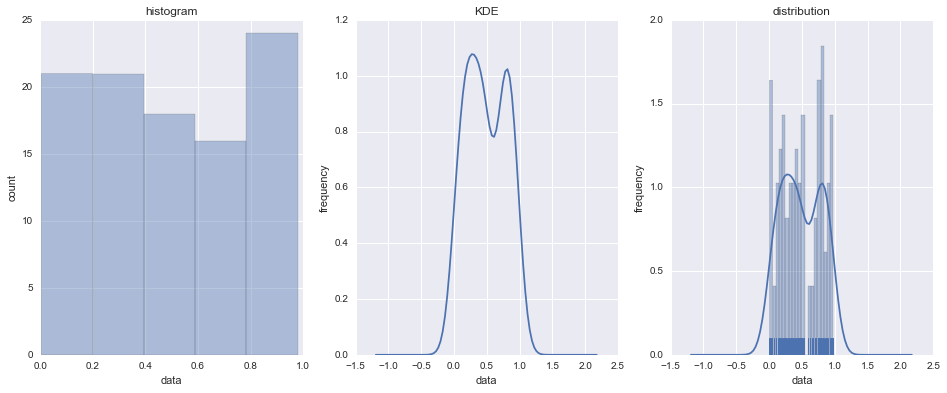
\includegraphics[height=0.15\textheight]{images/ex1}
        \item Grammar of Graphics\\
          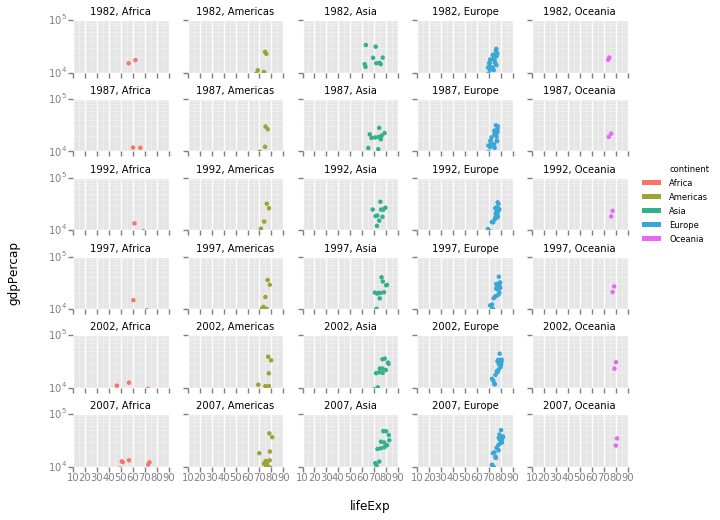
\includegraphics[height=0.15\textheight]{images/ex3}          
        \item Interactive map with bokeh\\
          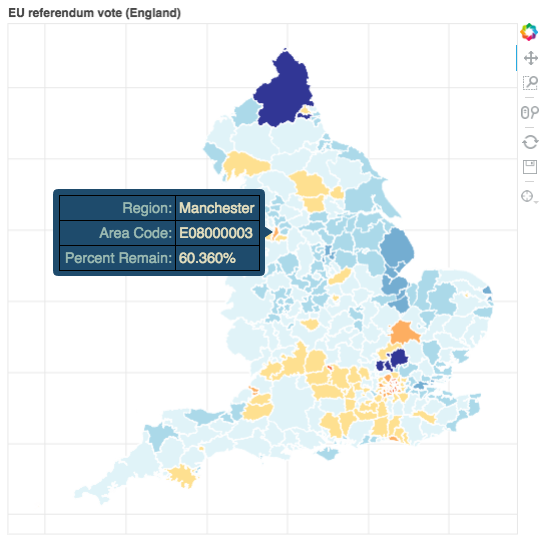
\includegraphics[height=0.15\textheight]{images/ex5}          
      \end{itemize}  
    \end{column}
    \begin{column}{5.5cm}  
      \begin{itemize}
        \item Two-variable, continuous x, y data\\
          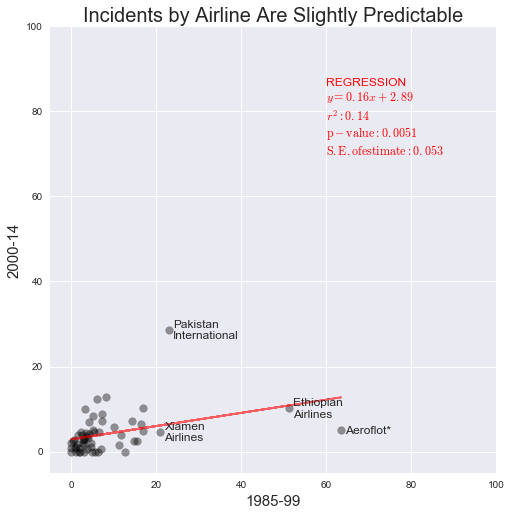
\includegraphics[height=0.15\textheight]{images/ex2}
        \item Arrays, colormaps, surface plots\\
          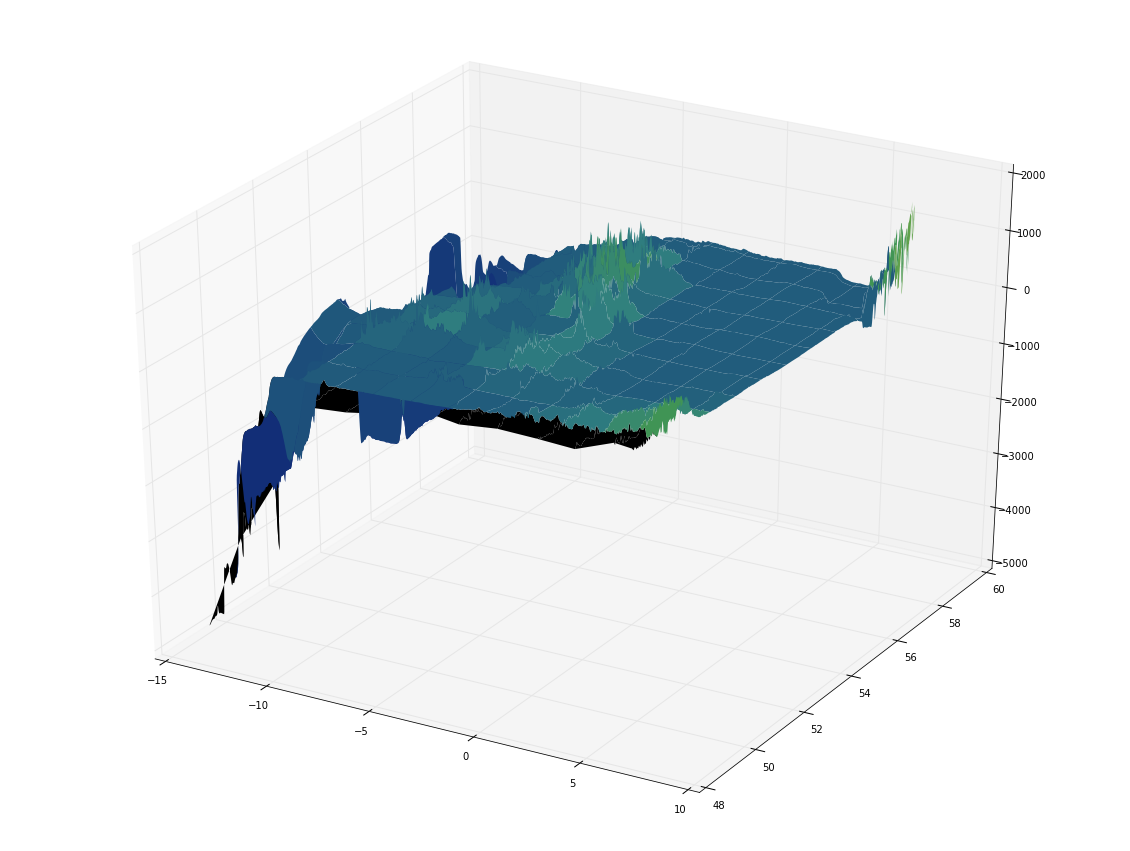
\includegraphics[height=0.15\textheight]{images/ex4}          
        \item Making movies\\
          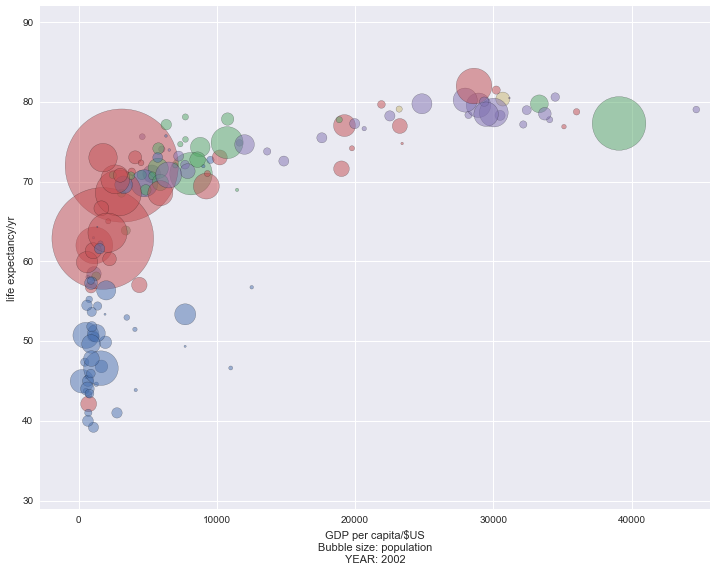
\includegraphics[height=0.15\textheight]{images/ex6}
      \end{itemize}
    \end{column}
  \end{columns}   
  \end{scriptsize}   
\end{frame}
